\graphicspath{{images/}}

\section{Background of Research}
\label{sec:background}

\subsection{A Comparison of Methods for Screening Strain Fitness }


% \begin{figure*}
%   \centering
%   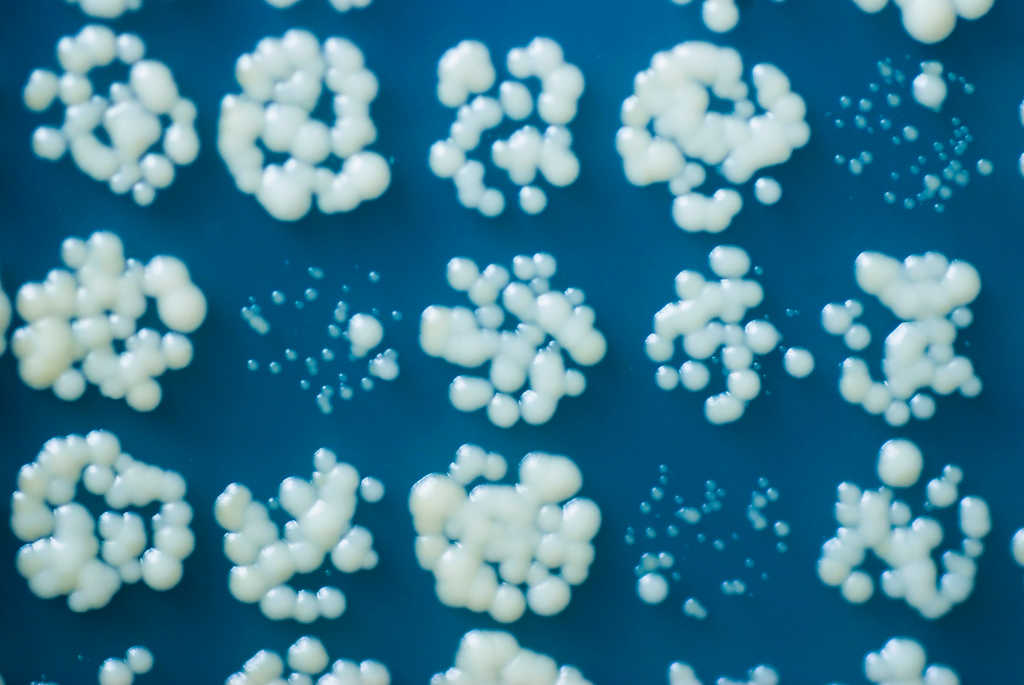
\includegraphics[width=\linewidth]{5658435523_c2e43729f1_b}
%   \captionof{figure}{An example QFA agar.}
% \end{figure*}

\begin{Figure}
  \centering
  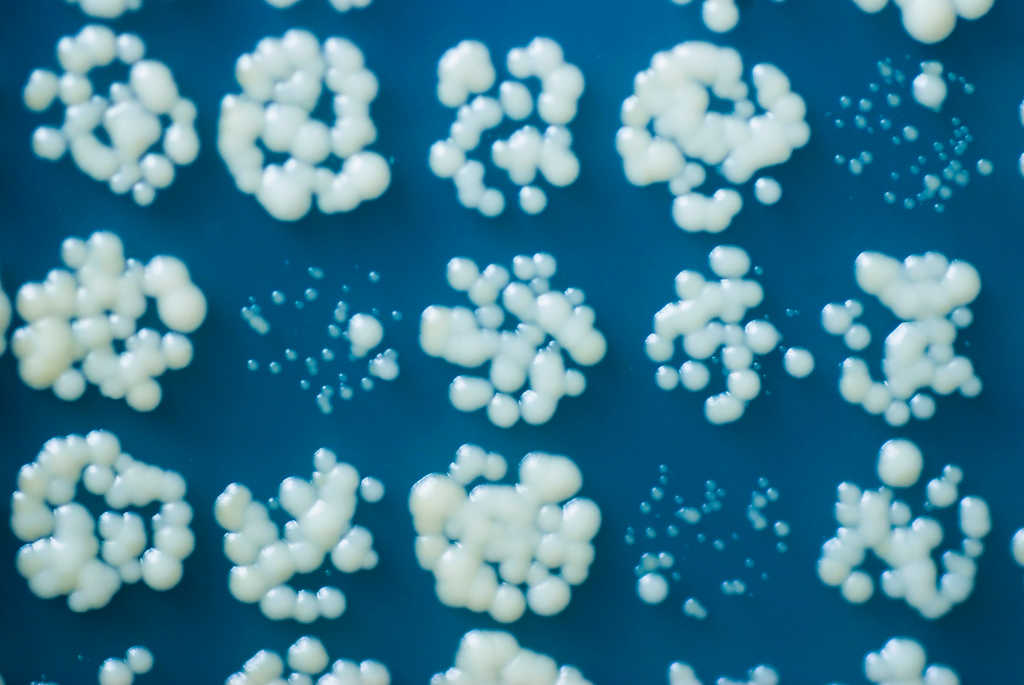
\includegraphics[width=\linewidth]{5658435523_c2e43729f1_b}
  \captionof{figure}{An example QFA agar.}
\end{Figure}


\begin{Figure}
  \centering
  %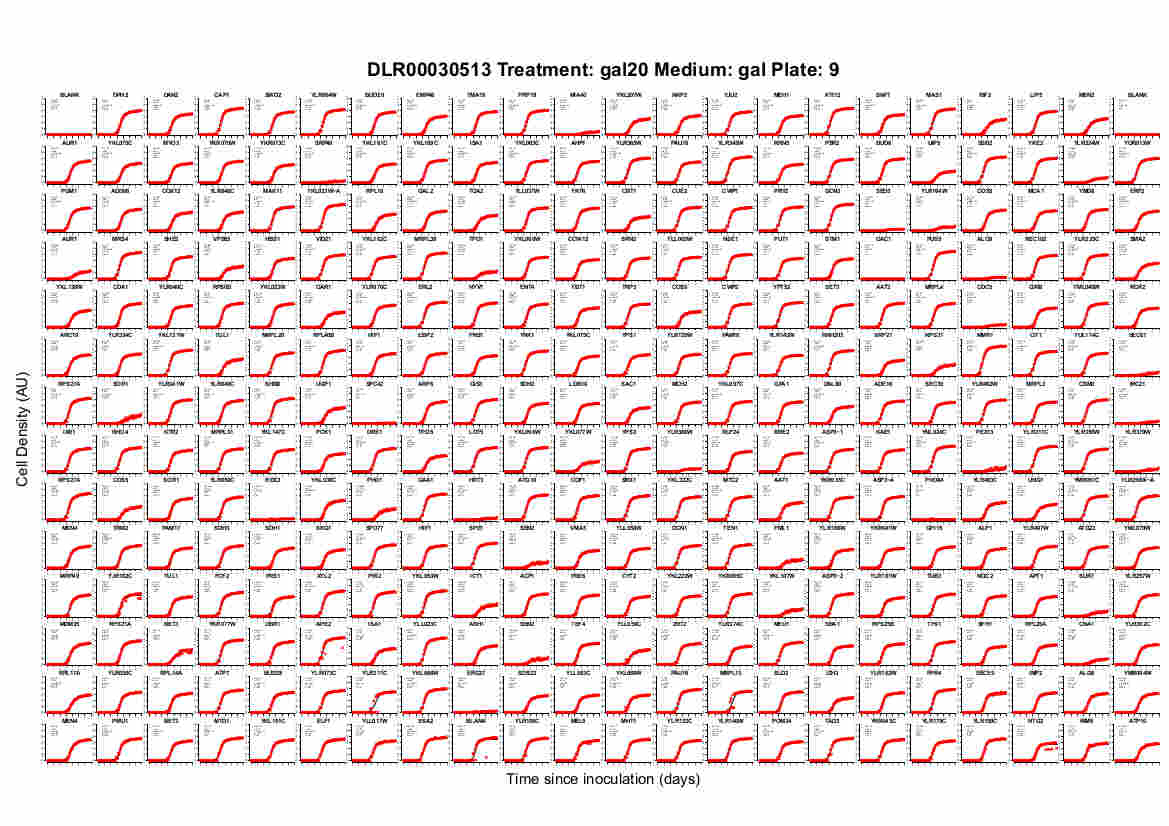
\includegraphics[width=\linewidth]{qfa_growth_array}
  \captionof{figure}{Growth curves of 308 genetic colonies from a FA. From (ref)}
\end{Figure}

\begin{Figure}
  \centering
  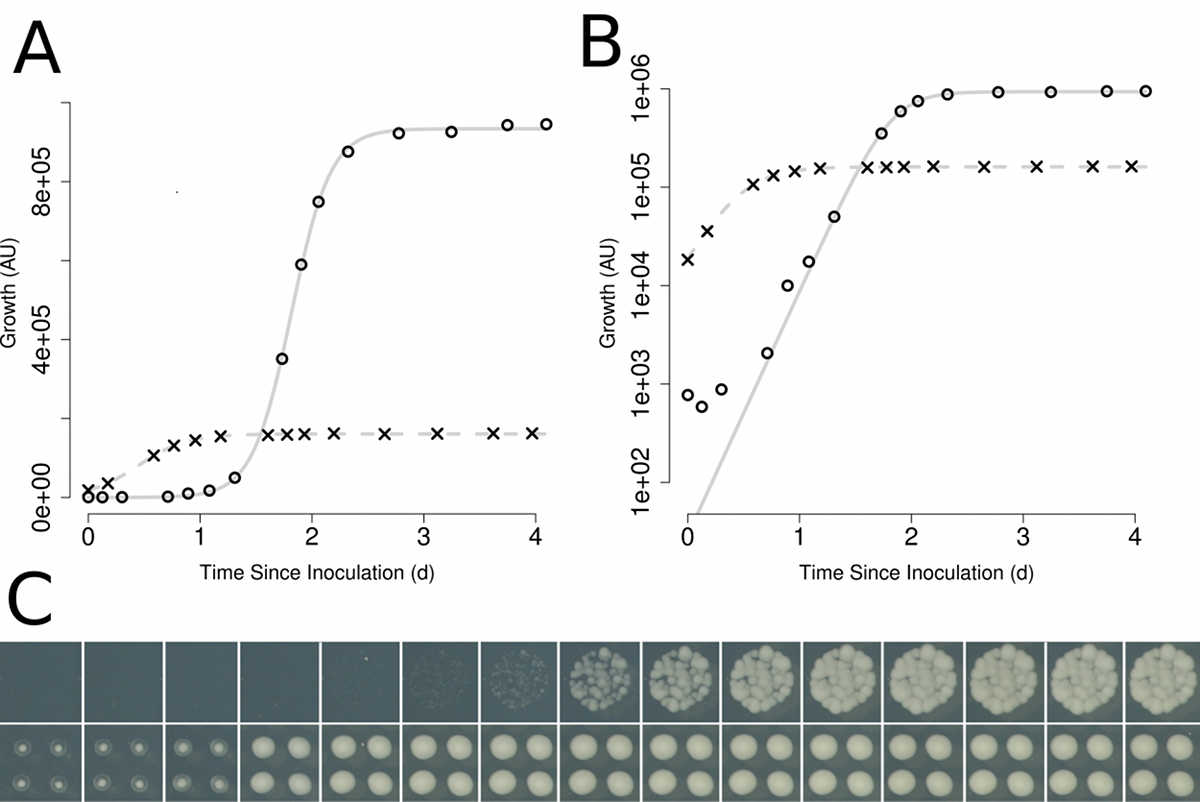
\includegraphics[width=\linewidth]{pin_v_spot_growth}
  \captionof{figure}{Pin v spot growth curves \citep{Lawless2010}.}
\end{Figure}


\subsection{Evidence of Competition and Signalling}

\subsection{Modelling Approaches}

\subsubsection{Mass Action Kinetics}
\subsubsection{The Logistic Growth Model}
\subsubsection{Fishers multiplicative model of }

\subsection{Inference of Genetic Interactions / Telomere Cap Defects}


%%% Local Variables:
%%% mode: latex
%%% TeX-master: "proposal"
%%% End:
